To evaluate our algorithm's performance a number of experiments were run on both the Euler and the Piz Daint cluster. In the following paragraphs we will first describe both the Euler and the Piz Daint setups. We will then go on to discussing each experiment.

\mypar{Euler setup} 
Each node in the Euler V cluster contains two 12-core Intel Xeon Gold 5118 processors and 96 GB of DDR4 memory clocked at 2400 MHz \cite{Euler}. We were allowed to use up to two nodes, giving us a maximum of 48 cores.

\mypar{Piz Daint setup} [Insert Daint specs]

\mypar{Graph Generation}
Our algorithm was evaluated on undirected, unweighted graphs. Multiple edges connecting the same two vertices and self loops were not allowed. All graphs were generated using \cite{Parmat}.

\mypar{MPI vs OMP vs Communication Avoiding}
The results in \autoref{fig:mpi_omp_commavoiding_euler} show our algorithm compared with the communication avoiding algorithm \cite{comm_avoiding} on three different graphs with the same number of edges but different densities. Our algorithm was run in MPI and OMP only mode.\\
\autoref{fig:mpi_omp_commavoiding_euler_1} shows the MPI only version outperforming the OMP version by a large margin on the densest graph. This can be explained by the combination of two effects: the first being that a dense graph results in more contention between the OMP threads during the edge contractions, and the second being that the reduction after the contractions scales linearly with the number of vertices. Since the number of vertices is comparatively low in a dense graph the reduction is fast. For the OMP only version we further observe a significant increase in total compute time from one to two cores and from 12 to 13 cores. The first jump can be explained by the initial overhead of doing the computation in parallel. Since a single CPU on Euler has 12 cores the second jump is a result of the cache coherency protocol being slow across multiple CPUs.\\
The results in \autoref{fig:mpi_omp_commavoiding_euler_2} and \autoref{fig:mpi_omp_commavoiding_euler_3} were obtained using sparser graphs compared to \autoref{fig:mpi_omp_commavoiding_euler_1}. Here, for a large number of cores, the OMP only version is clearly faster than the MPI only version. \autoref{fig:mpi_omp_commavoiding_euler} shows a trend of the OMP only version speeding up as the graph becomes sparser, while the MPI only version slows down. The OMP only version's speed up can be explained by the reduced contention between the OMP threads due to the sparser graph. The MPI only version's slow down is a result of the increased reduction time due to the increasing number of vertices.\\
The results in \autoref{fig:mpi_omp_commavoiding_euler} show the communication avoiding algorithm scaling badly with the number of cores. This is expected since the edge contractions are computed on a single node in this algorithm. Since our algorithm does to scale with the number of cores up to some point we manage to outperform the communication avoiding algorithm on each graph.

\begin{figure}
\begin{subfigure}[c]{0.15\textwidth}
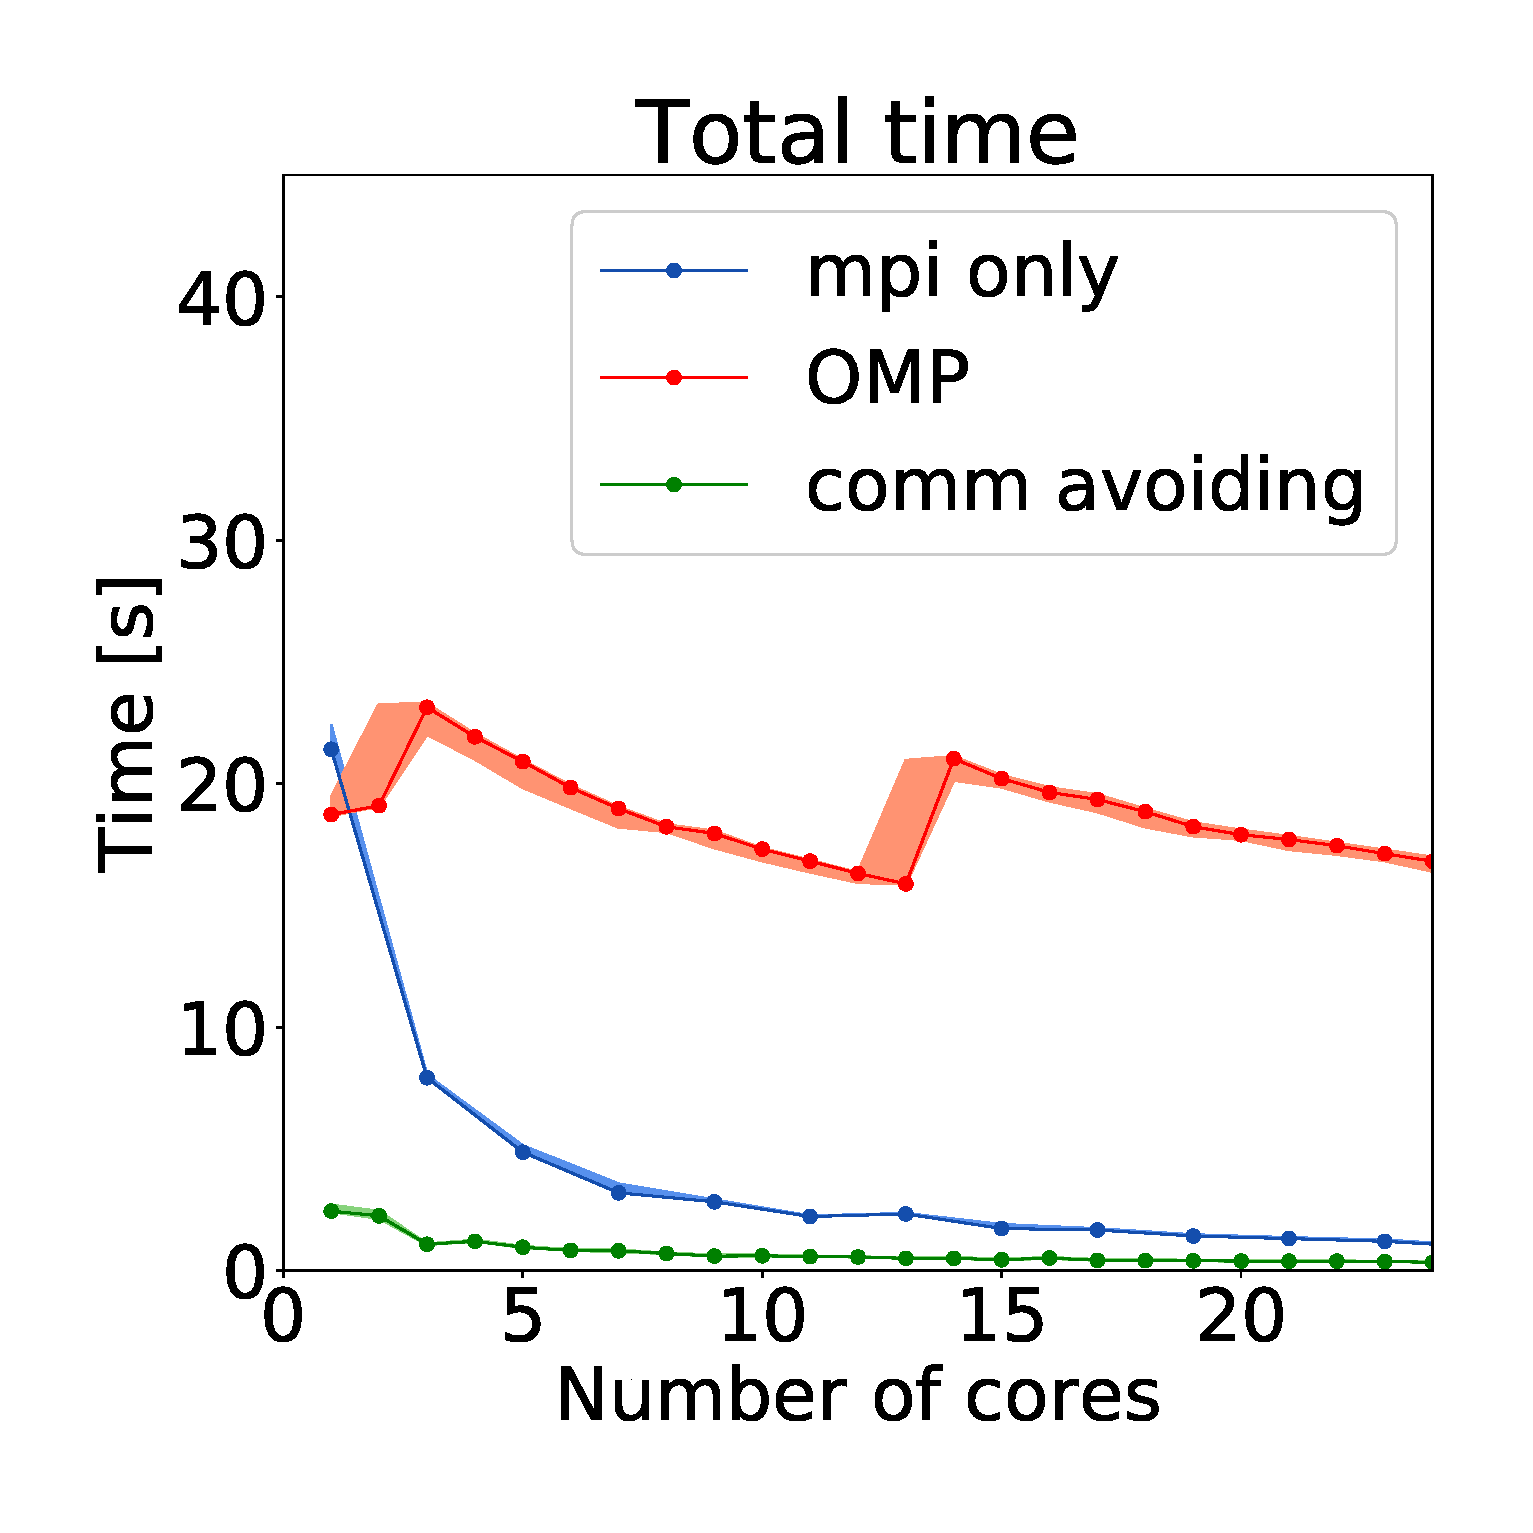
\includegraphics[width=\textwidth]{plots/50000our_impl}
\subcaption{$5\times10^{5}$ vertices}
\label{fig:mpi_omp_commavoiding_euler_1}
\end{subfigure}
\begin{subfigure}[c]{0.15\textwidth}
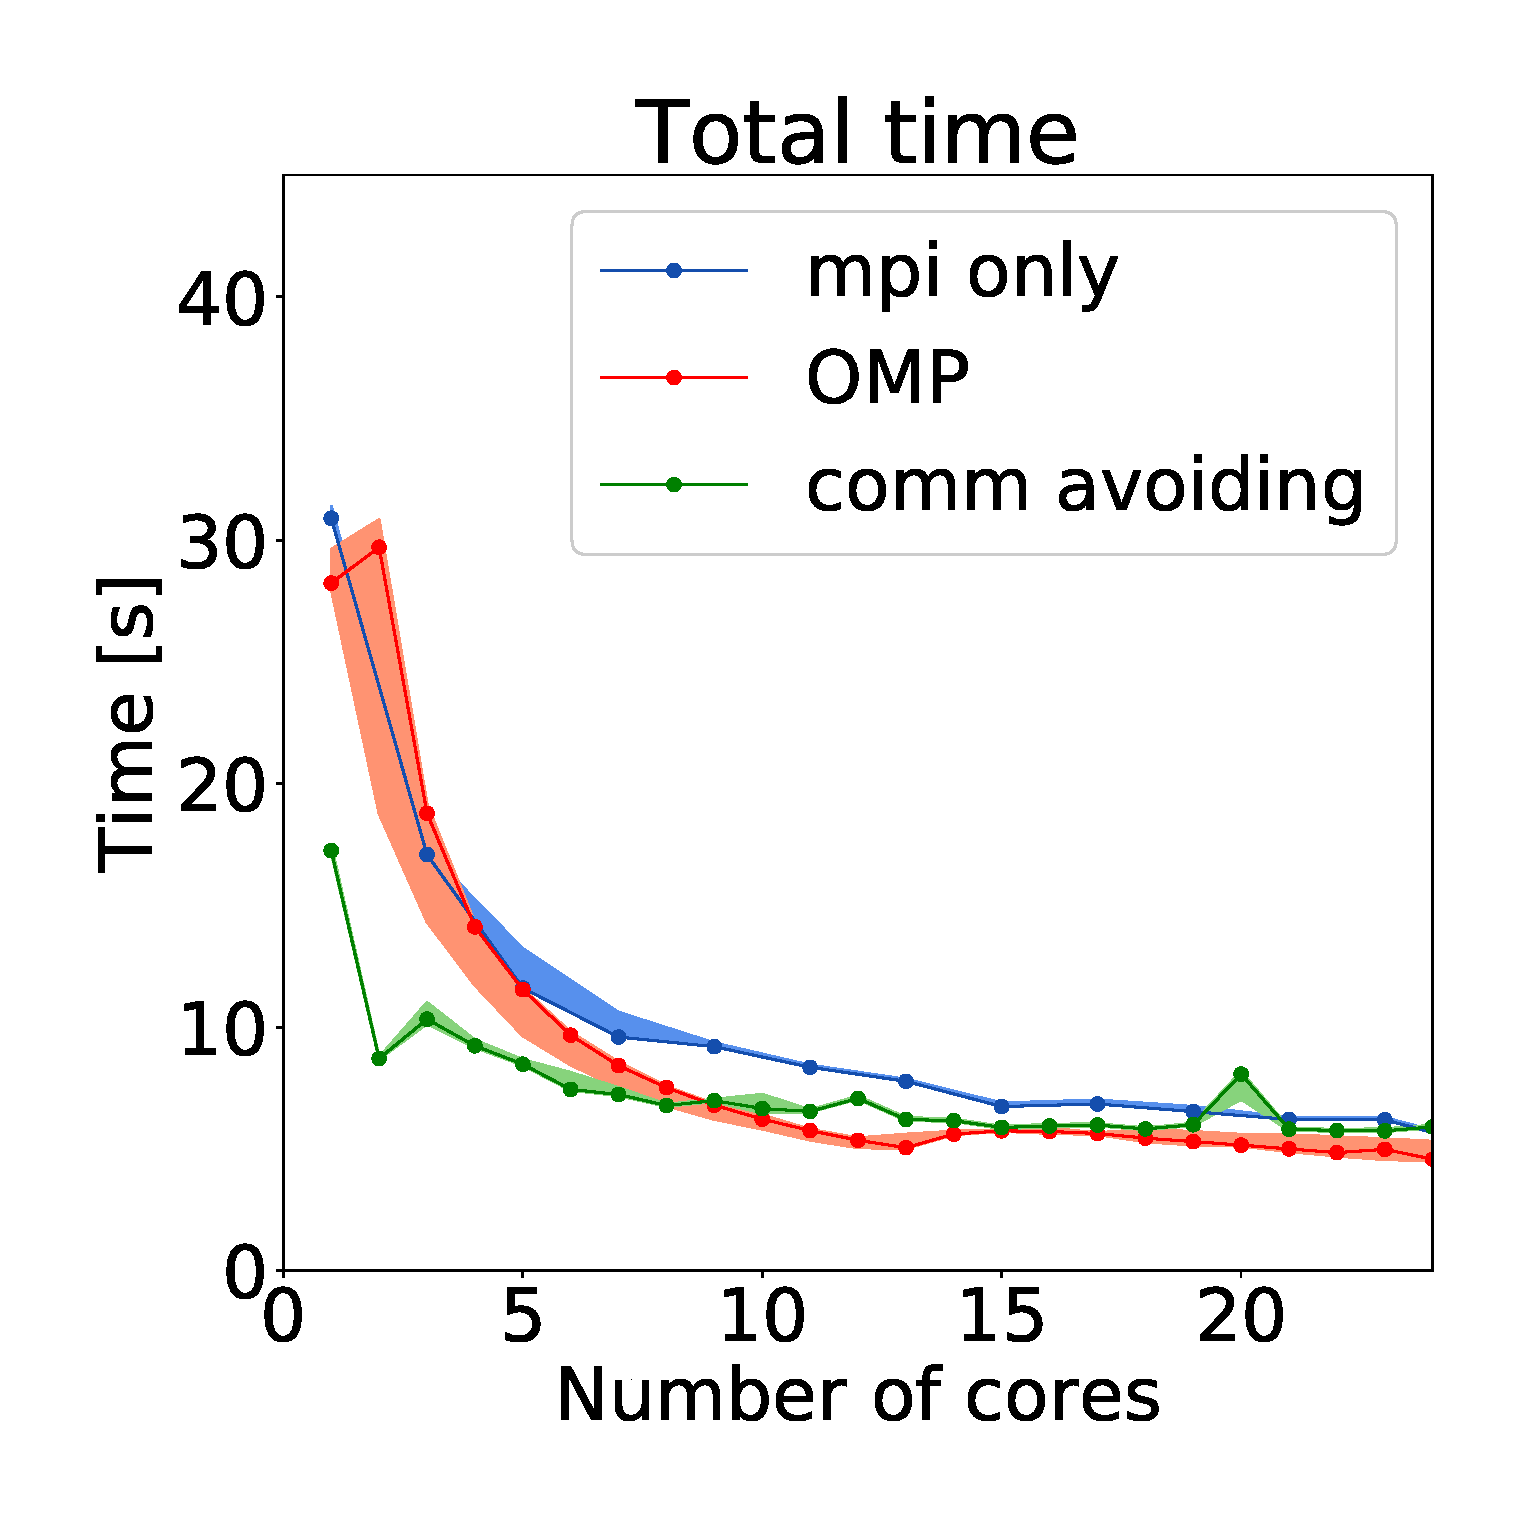
\includegraphics[width=\textwidth]{plots/10000our_impl}
\subcaption{$10^{7}$ vertices}
\label{fig:mpi_omp_commavoiding_euler_2}
\end{subfigure}
\begin{subfigure}[c]{0.15\textwidth}
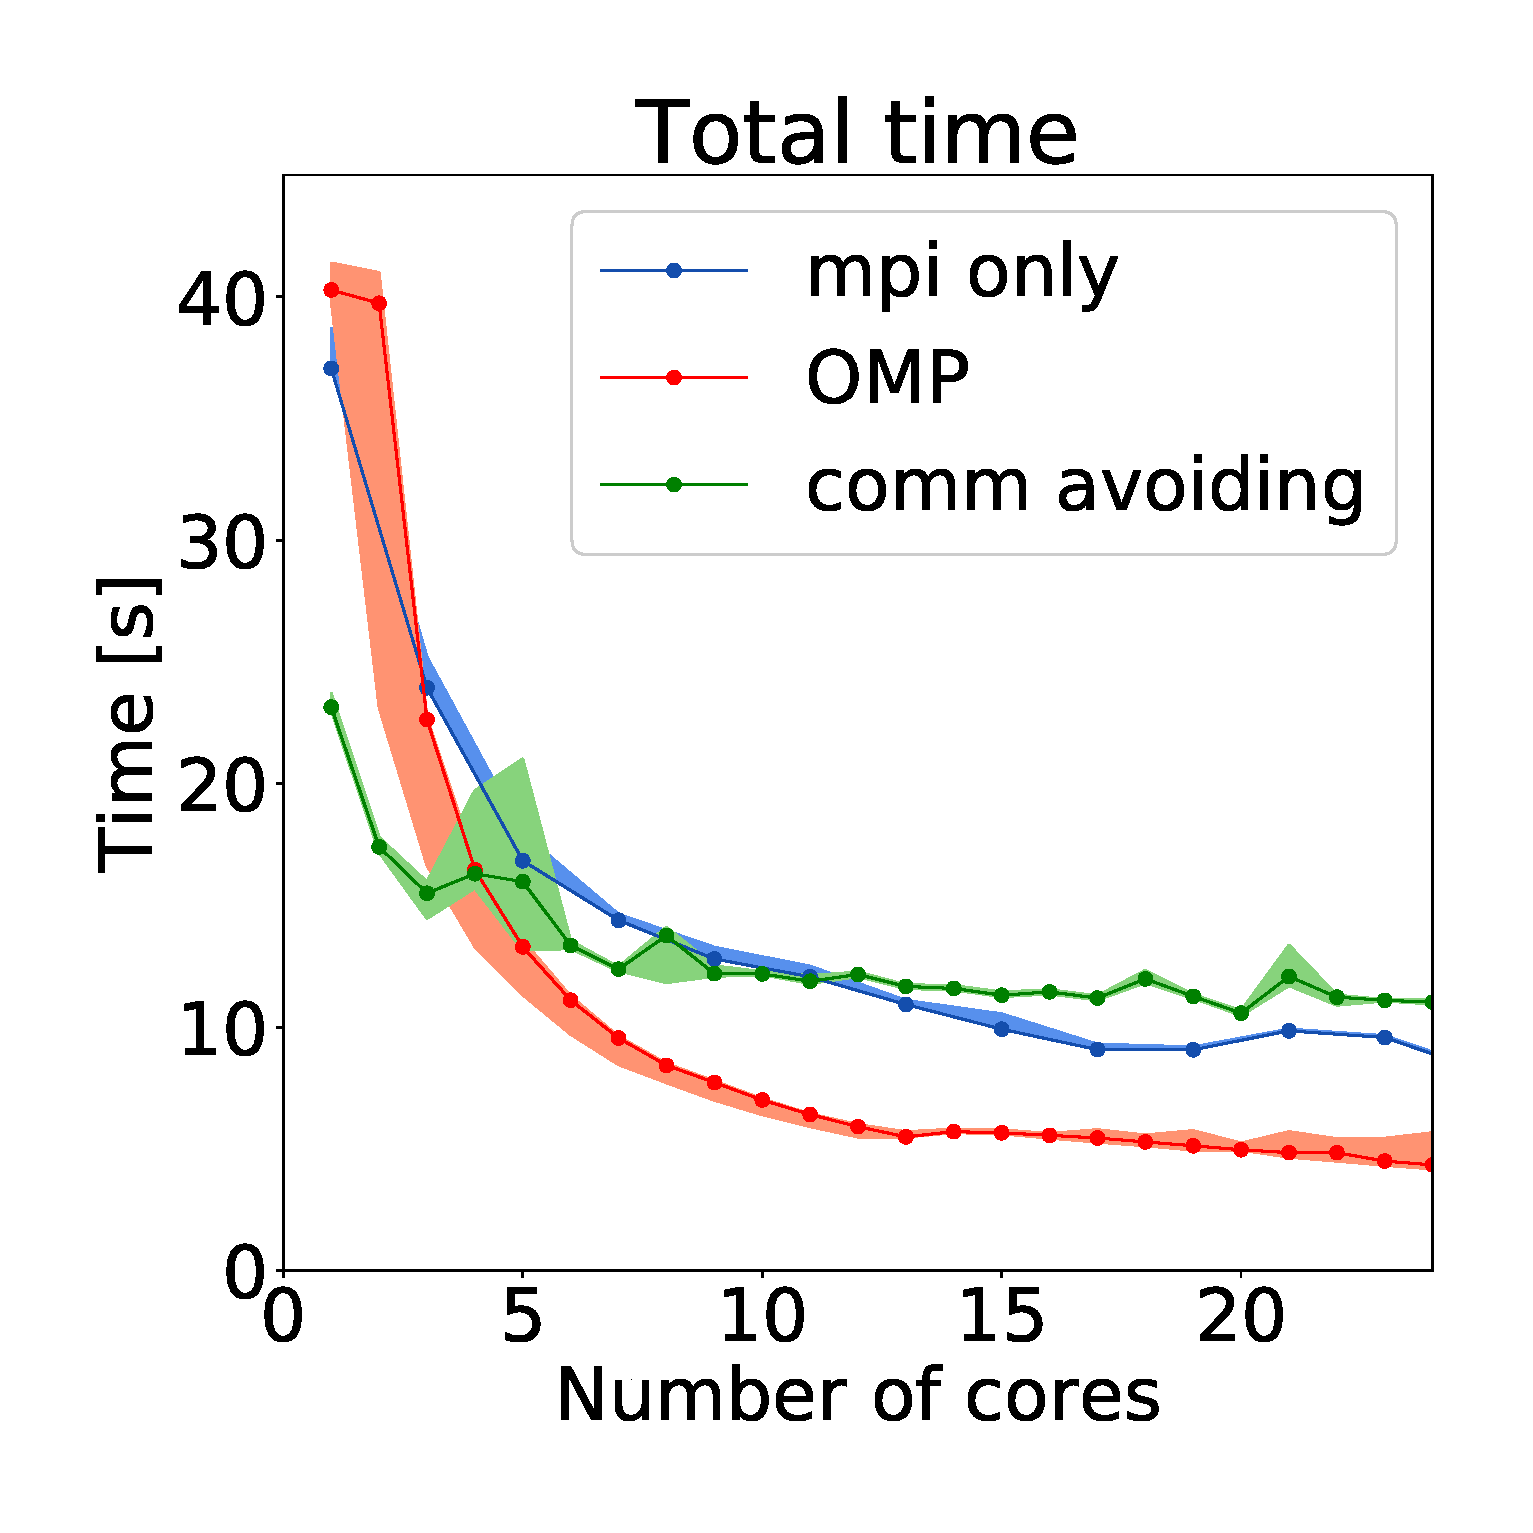
\includegraphics[width=\textwidth]{plots/20000our_impl}
\subcaption{$2\times10^{7}$ vertices}
\label{fig:mpi_omp_commavoiding_euler_3}
\end{subfigure}
\caption{Total runtime of three different graphs each with $5\times10^{8}$ edges. The experiment was run on the Euler cluster.}
\label{fig:mpi_omp_commavoiding_euler}
\end{figure}

\mypar{Mixing MPI and OMP}
To further investigate the distinct difference between the MPI only and the OMP only version the algorithm was tested using a mixture of MPI and OMP.

\begin{figure}
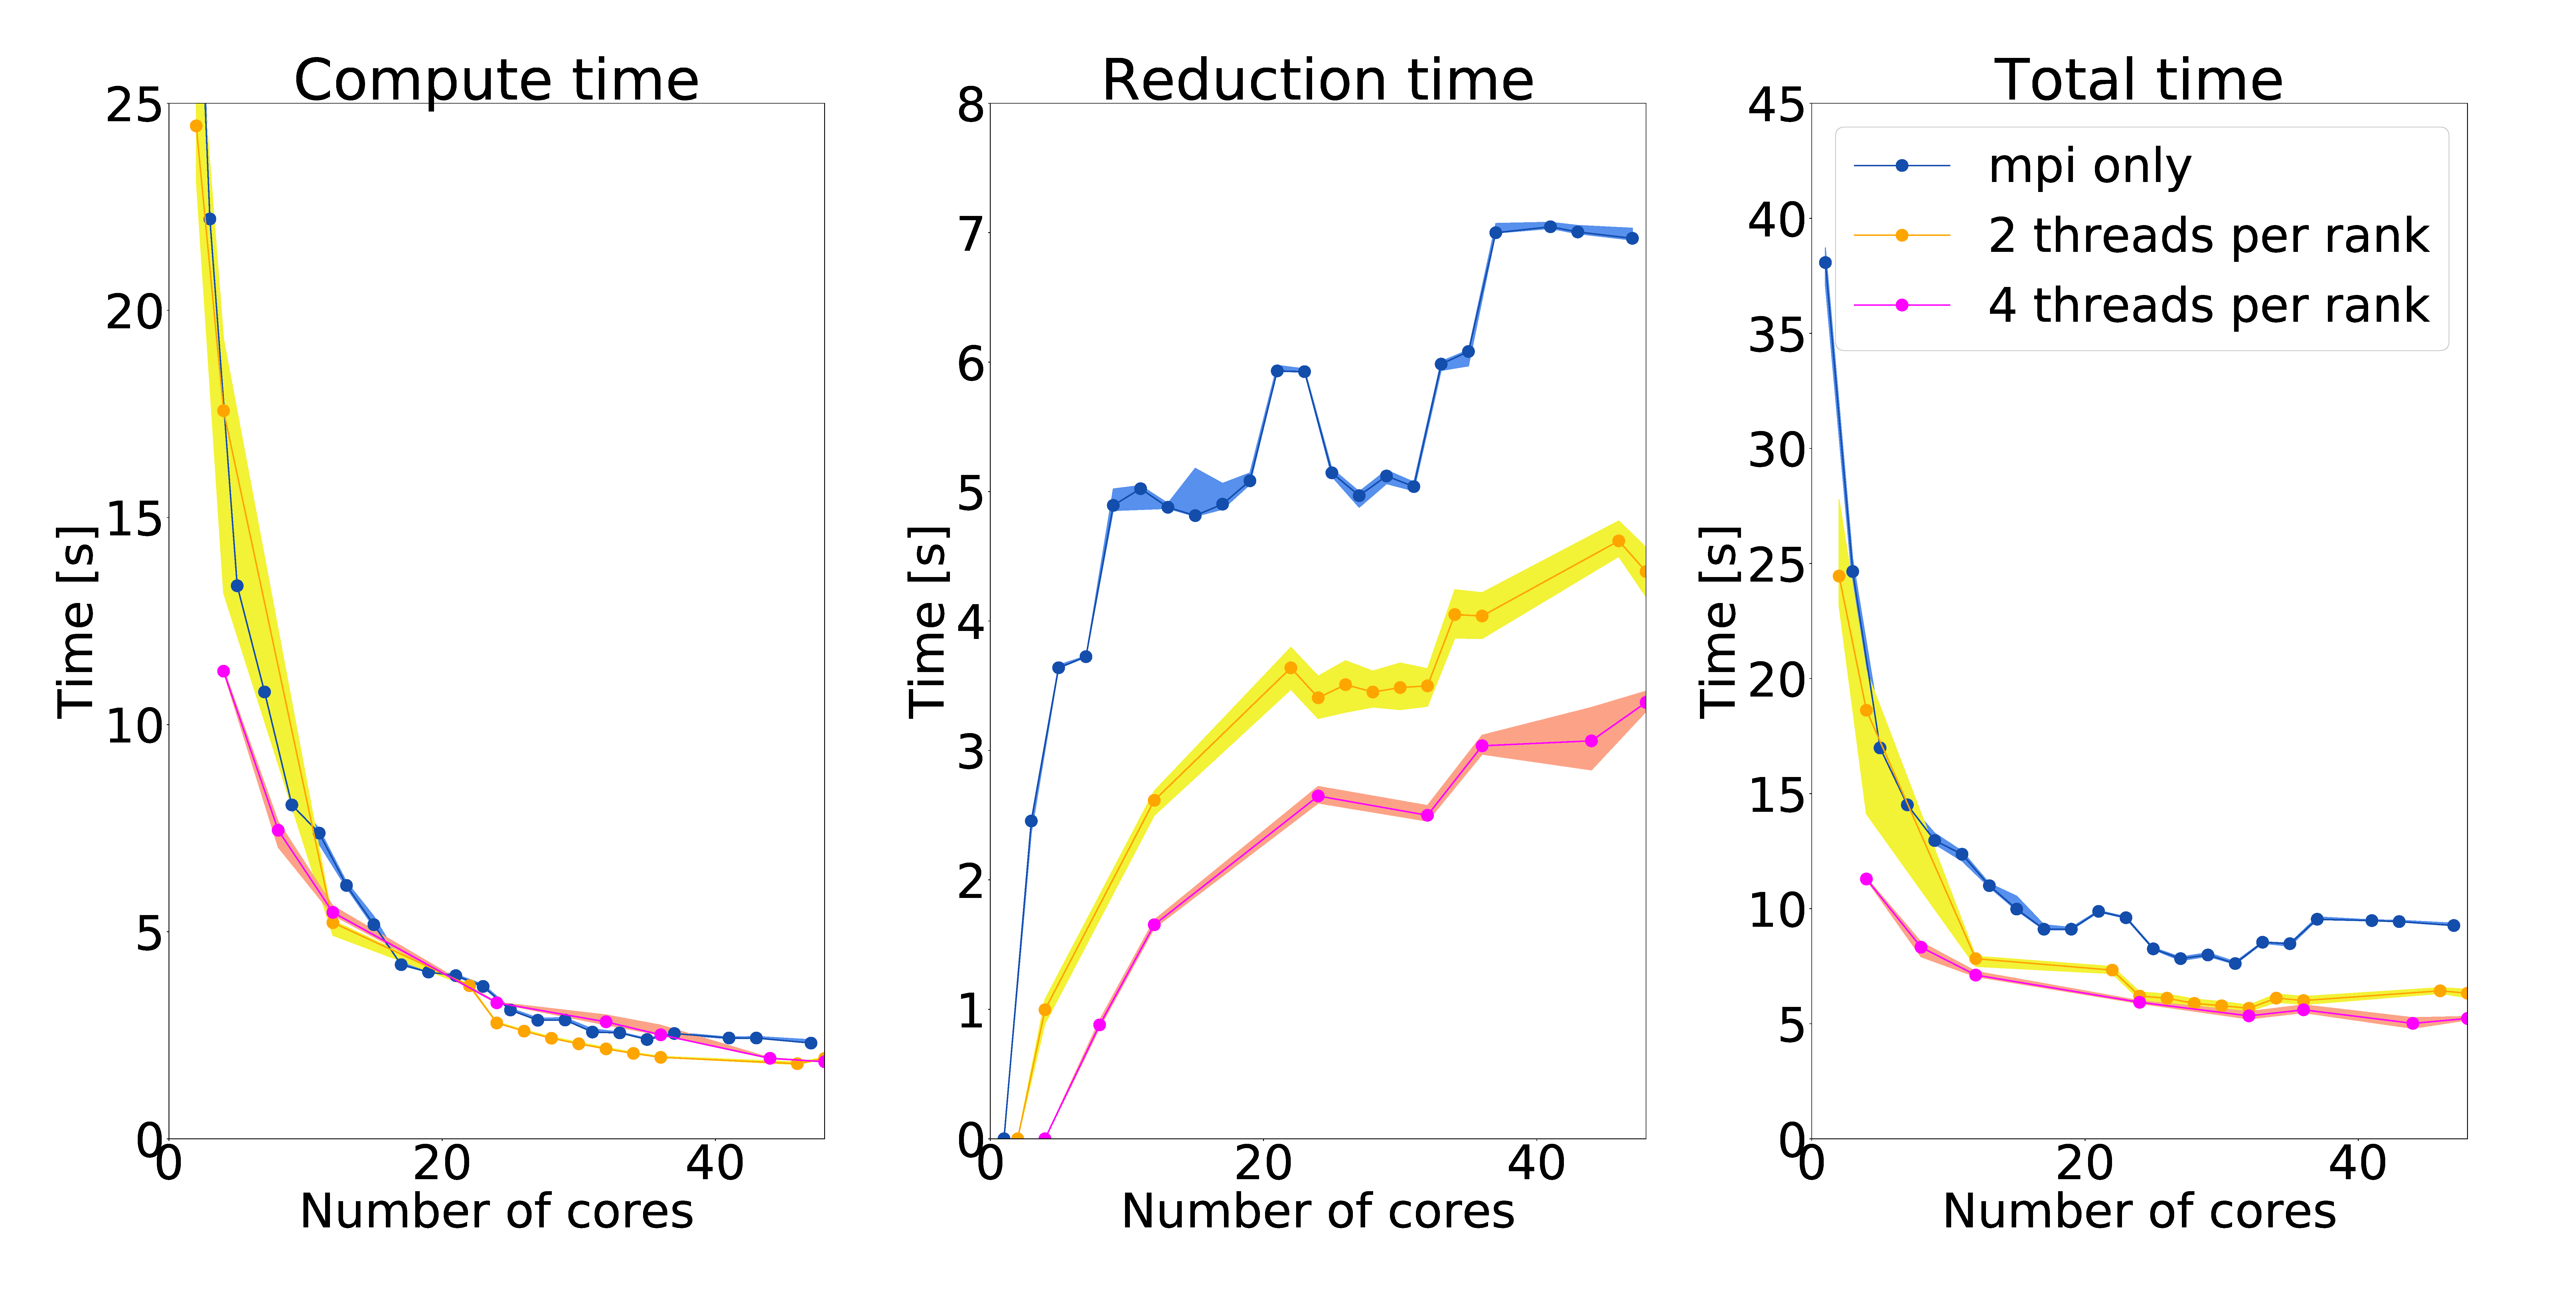
\includegraphics[width=0.5\textwidth]{plots/20000mpi_mixtures_with_everything}
\subcaption{$2\times10^{7}$ vertices}
\caption{Total runtime breakdown on graph with $5\times10^{8}$ edges and $2\times10^{7}$ vertices. The experiment was run on the Euler cluster.}
\label{fig:mixed_euler}
\end{figure}

\autoref{fig:mixed_euler} shows the compute time being largely independent of the mixture. This is a consequence of the graphs sparsity which results in low contention between the OMP threads. The reduction time, however, wildly differs for the different mixtures. For each mixture it increases logarithmically with the number of MPI ranks. This results in the algorithm's performance decreasing as less OMP threads per MPI rank are used.

\mypar{Speedups}

\begin{figure}
\begin{subfigure}[c]{0.23\textwidth}
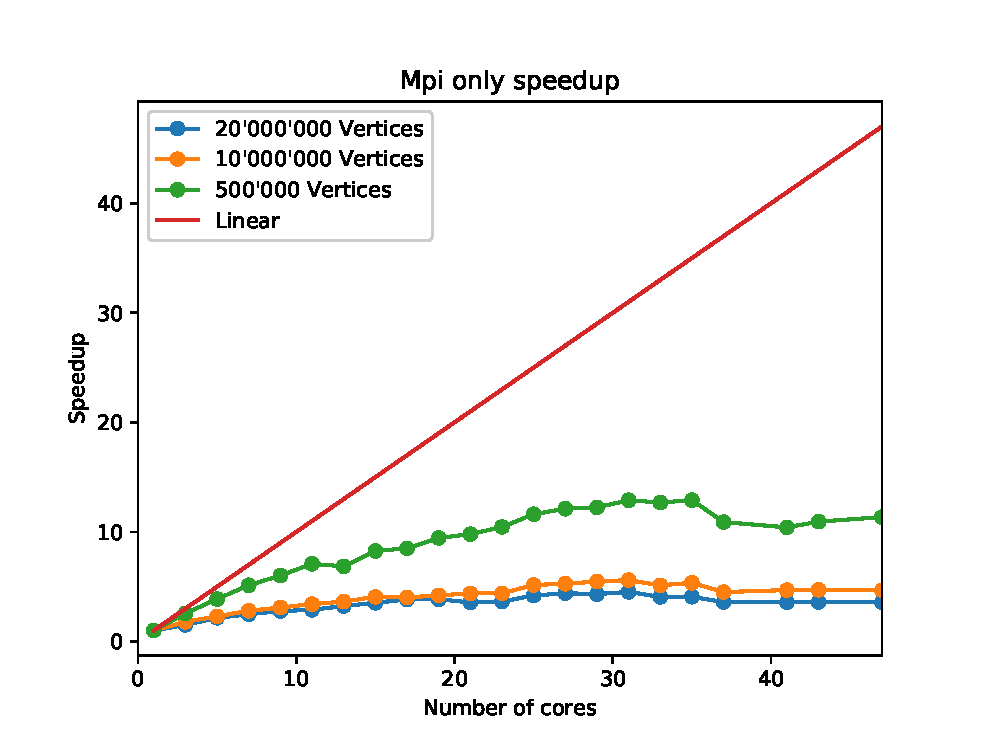
\includegraphics[width=\textwidth]{plots/mpi_speedup_with_ref}
\subcaption{MPI only}
\label{fig:speedup_mpi}
\end{subfigure}
\begin{subfigure}[c]{0.23\textwidth}
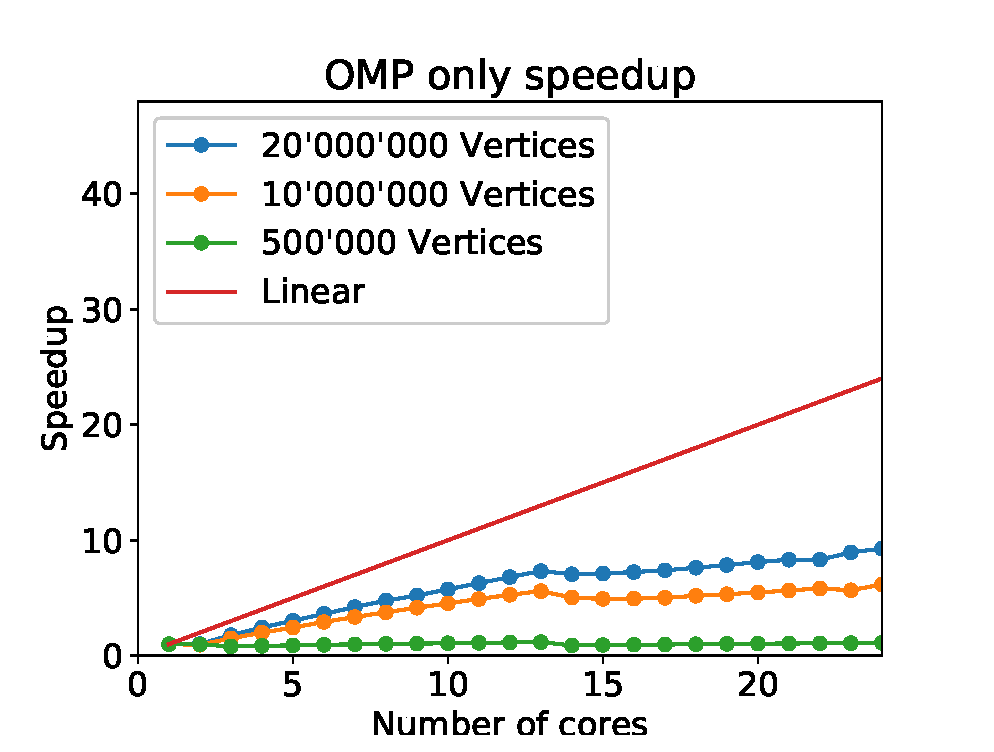
\includegraphics[width=\textwidth]{plots/omp_speedup_with_ref}
\subcaption{OMP only}
\label{fig:speedup_omp}
\end{subfigure}
\caption{Speedup of MPI only and OMP only version on three different graphs each with $5\times10^{8}$ edges.}
\label{fig:speedup}
\end{figure}

\autoref{fig:speedup} shows the measured speed up of the MPI only and OMP only version. As one would expect from the results discussed previously the MPI only version achieves better scaling compared to the OMP only version on dense graphs while the OMP only version scales better on sparse graphs.

